\subsubsection{Projeto Eletrônico}
% CIRCUITO ELÉTRICO/ELETRÔNICO COMPLETO
% MOSTRAR/EXPLICAR: PLACA DE CIRCUITO IMPRESSO DESENVOLVIDA
% TODO:
% ref:  https://produza.ind.br/gestao/pre-requisitos-tecnicos-para-montar-um-projeto-eletronico/

% \begin{figure}[H]
%     \centering
%     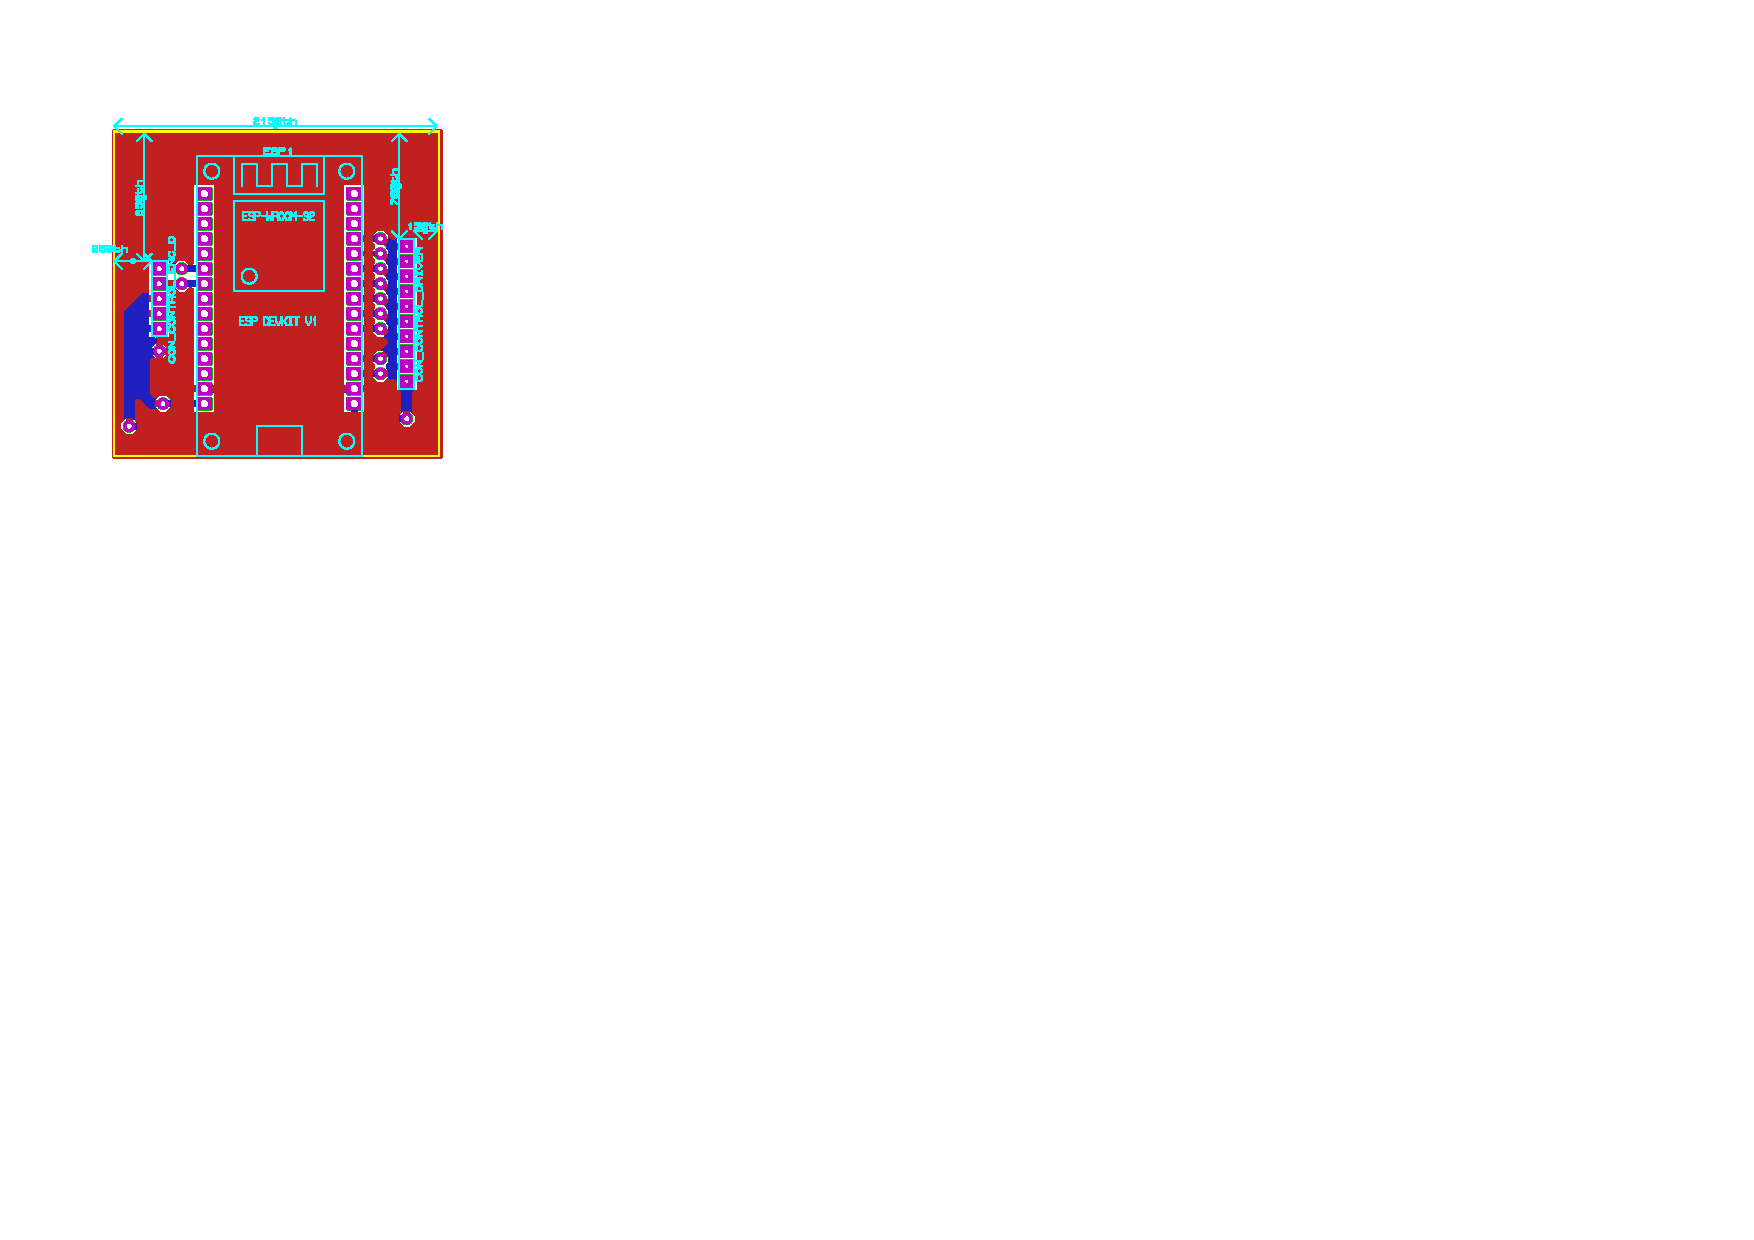
\includegraphics[width=\textwidth]{imagens/eletronica/placa/placa_controle_completa.pdf}
%     \caption{Caption}
%     % \label{fig:my_label}
% \end{figure}

% \begin{figure}[H]
%     \centering
%     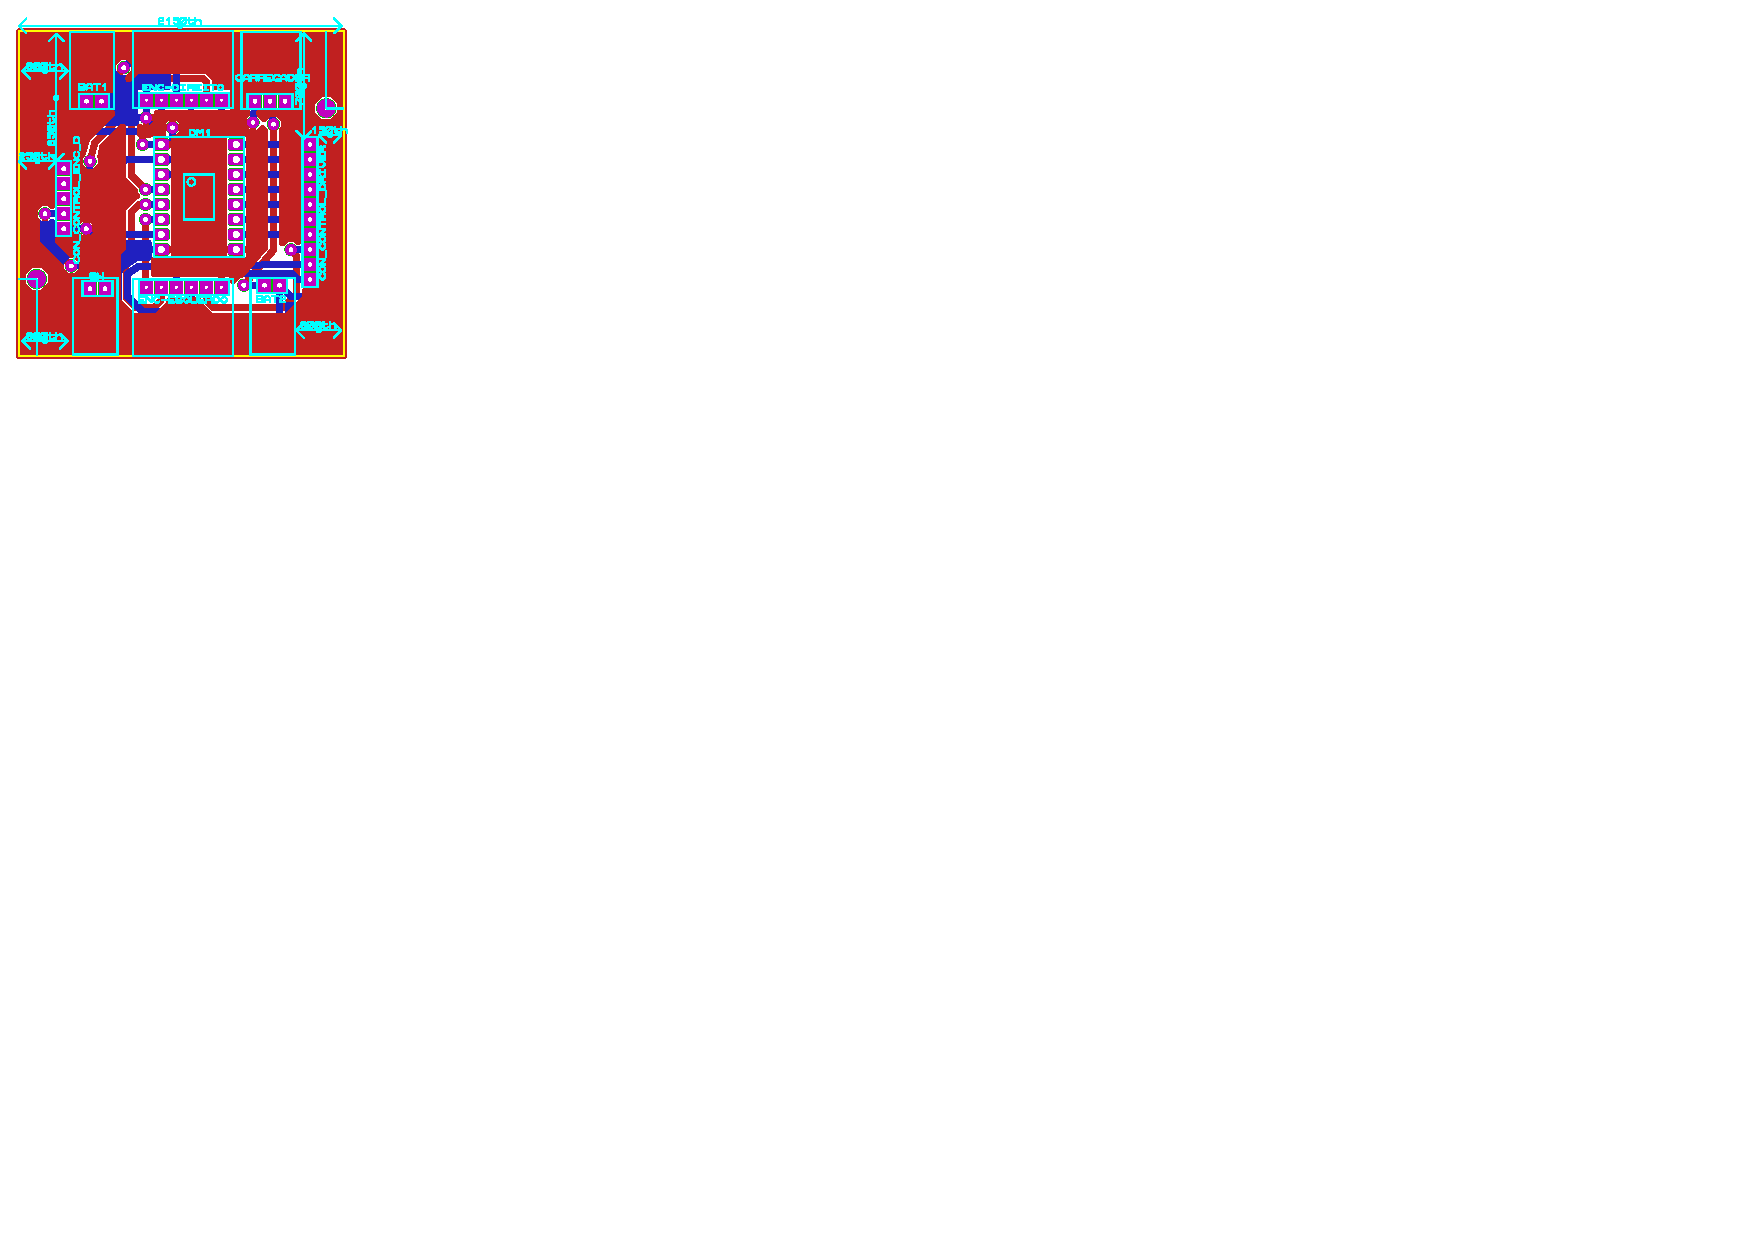
\includegraphics[width=\textwidth]{imagens/eletronica/placa/placa_driver_completa.pdf}
%     \caption{Caption}
%     % \label{fig:my_label}
% \end{figure}

\begin{enumerate}
    \item \textbf{Concepção inicial}:
        O principal objetivo por trás de se fazer uma nova placa de circuito eletrônico é acomodar os componentes, respeitando os limites das dimensões estabelecidos pela competição na qual os robôs serão utilizados (caber dentro de um cubo de $75$ mm de aresta). A placa deve conter o microcontrolador, no seu kit de desenvolvimento, \textit{Driver motor} para acionamento dos motores DCs, os \textit{Encoders} e ser alimentada por duas baterias de $1$ célula do tipo \textit{Lipo}.
        
    \item \textbf{Elaboração dos esquemáticos eletrônicos}:
        O esquemático foi a parte mais simples, pois não houve grandes mudanças nessa parte, com relação aos projetos de anos anteriores. A maior mudança foi o microcontrolador, que provocou dificuldades maiores na etapa seguinte, a elaboração do \textit{Layout}, devido às dimensões dos componentes.
        
        % inserir imagem do esquemático geral aqui
        
        \begin{figure}[H]
            \centering
            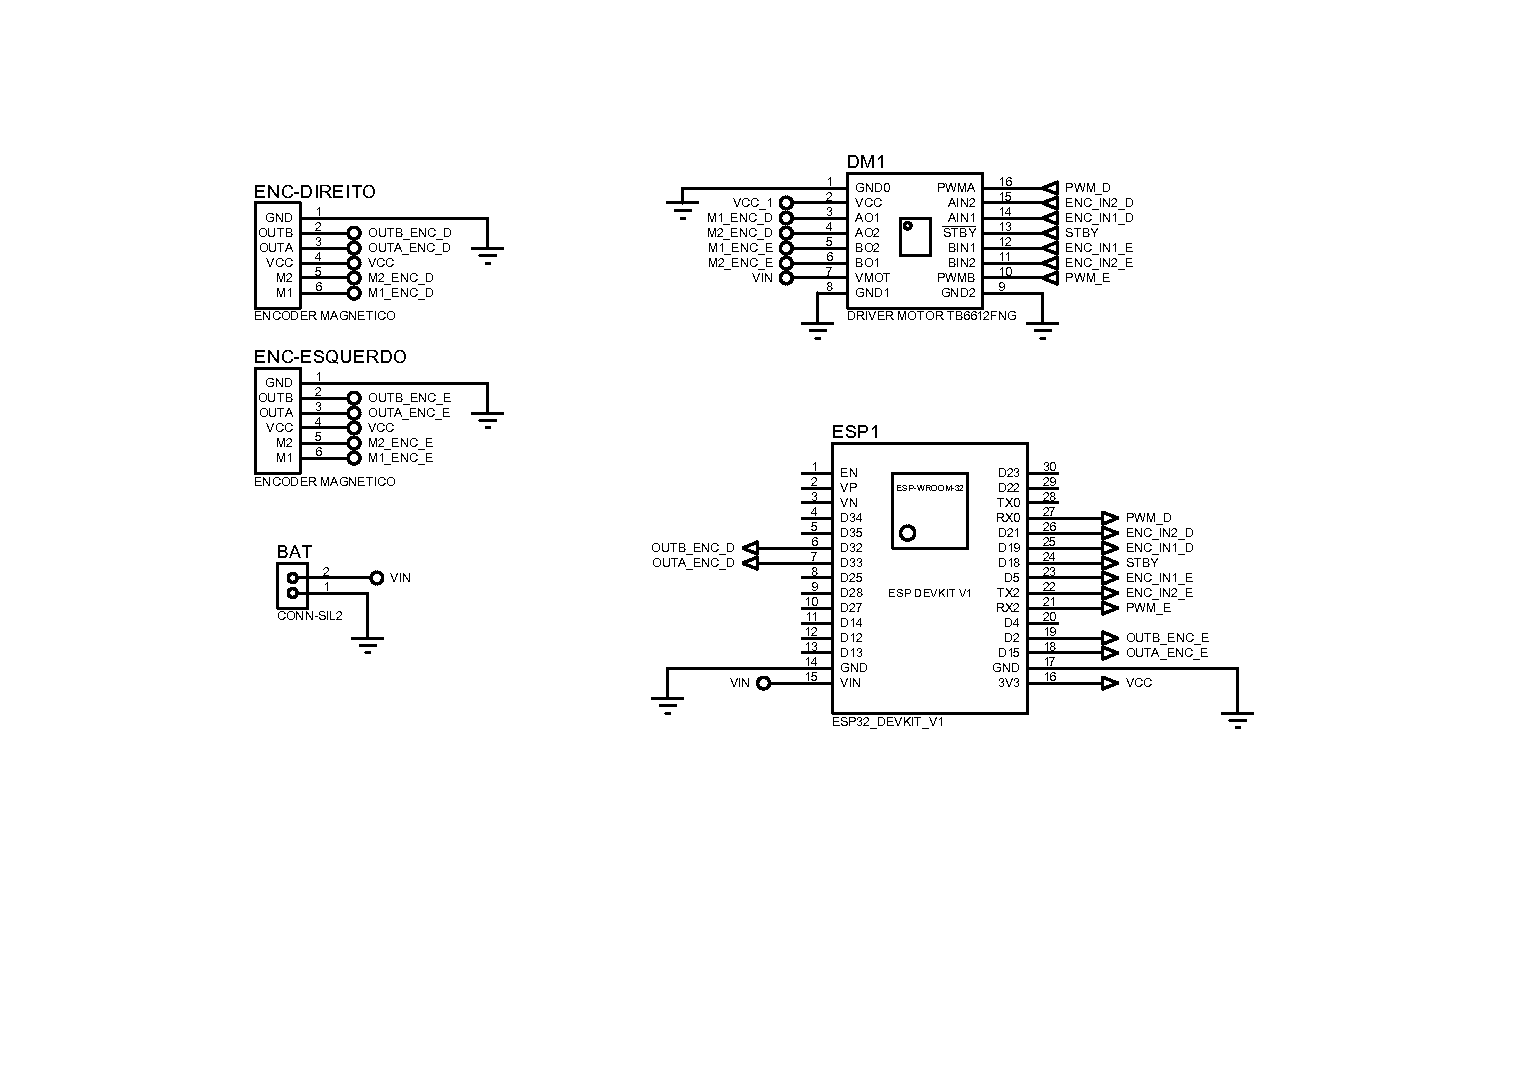
\includegraphics[width=\textwidth]{imagens/eletronica/placa/esquematico_completo.pdf}
            \caption{Esquemático.}
        \end{figure}
        
    \item \textbf{Elaboração do layout}:
        % inserir imagem do layout final aqui
        Este ponto foi o mais crítico nessa tarefa, devido à restrição de tamanho da placa ser de um quadrado com até $55$mm de lado. A solução adotada foi fazer em duas camadas, ou seja, duas placas cobreadas, ambas dupla face, dividindo os componentes. Em uma placa foi comportado o \textit{Driver}, bem como os conectores para os motores com os sensores e os conectores das baterias, e na outra apenas o microcontrolador. Para a conexão entre as placas foi utilizado um conector do tipo \textit{Head}, um macho e uma fêmea. Dessa forma, as placas conseguiram respeitar o limite dimensional e comportar todos os componentes necessários.
    \item \textbf{Realização de testes}:
        % faltou imagem de testes aqui
        Foram realizados testes antes da concepção da PCI, em \textit{Protoboards} para conferir se o circuito está funcionando como esperado e após a confecção, para se verificar a qualidade da confecção das placas.
        
        Também foram realizados testes individuais nos componentes, principalmente nos sensores, com o uso de osciloscópios. Verificou-se o funcionamento correto dos \textit{Encoders} e também conferiu-se se a distância entre os sensores poderia estar gerando interferência um no outro. Os resultados desses testes foram que todos os \textit{encoders} utilizados estão em bom estado, ou seja, funcionando como esperado e a distância que eles ficarão ao serem acomodados na estrutura não causa interferência um no outro.
    \item \textbf{Verificação e validação}
        Após testes individuais, de cada componente, foram realizados testes com a montagem completa, ou seja, os robôs montados por completo com as PCIs, baterias, motores e sensores. A validação foi por meio de controle manual dos robôs e testes simples de leitura de \textit{Encoder}, pois nessa etapa o \textit{Firmware} ainda não havida sido implementado.
\end{enumerate}